\chapter{I2C GPIO/Multiplexer}
\chaplabel{i2cgpio}

\section{Introduction}
This chapter introduces students to using the PCA9535 I$^2$C GPIO chip to control LEDs and input button 
presses. The PCA9535 has 16 I/O pins that are controlled via I$^2$C. It's I$^2$C address can be set 
between 0x20 and 0x27 through setting the A0-A2 pins either high (1) or low (0). These pins control 
the lower 3 bits of the address. The two 8-bit I/O pin ports (IO0 and IO1) are controlled via a set of 
eight registers. Registers are binary numbers where each bit sets the configuration of one of the I/O pins.

\section{Registers}
\subsection{Registers 0 and 1 - Input Registers}
These registers reflect the incoming logic levels of the port pins no matter whether the port is 
configured as an input or an output. These ports are read only; you cannot write to them. 
Table~\ref{table:pca9535inputports} shows the registers.

\begin{table}[!htb]
	\centering
	\begin{tabular}{l c c c c c c c c}
        \multicolumn{5}{l}{\textbf{I/O Input Register Port 0}} \\
		\hline
		Bit & 7 & 6 & 5 & 4 & 3 & 2 & 1 & 0 \\
		\hline
        Symbol & I0.7 & I0.6 & I0.5 & I0.4 & I0.3 & I0.2 & I0.1 & I0.0\\
        Default & X & X & X & X & X & X & X & X \\
        \hline
        \\
        \multicolumn{5}{l}{\textbf{I/O Input Register Port 1}} \\
		\hline
		Bit & 7 & 6 & 5 & 4 & 3 & 2 & 1 & 0 \\
		\hline
        Symbol & I1.7 & I1.6 & I1.5 & I1.4 & I1.3 & I1.2 & I1.1 & I1.0\\
        Default & X & X & X & X & X & X & X & X \\
        \hline
	\end{tabular}
	\caption{PCA9535 input port values are shown here. The Default value of X means 
    that it's value is not set at power on. Also, note that the Port 0 symbols are the 
    letter I followed by the number zero, not the letter O.}
	\label{table:pca9535inputports}
\end{table}


\subsection{Registers 2 and 3 - Output Registers}
These registers control the output value of the pins that are set as outputs. Pins are set
as outputs or inputs in Registers 6 and 7. Note that the default output value of all the 
pins is 1 or logic high. It is important to note that the values in these registers have 
no effect on pins that are defined as inputs. Table~\ref{table:pca9535outputports} shows 
the registers.

\begin{table}[!htb]
	\centering
	\begin{tabular}{l c c c c c c c c}
        \multicolumn{5}{l}{\textbf{I/O Output Register Port 0}} \\
		\hline
		Bit & 7 & 6 & 5 & 4 & 3 & 2 & 1 & 0 \\
		\hline
        Symbol & O0.7 & O0.6 & O0.5 & O0.4 & O0.3 & O0.2 & O0.1 & O0.0\\
        Default & 1 & 1 & 1 & 1 & 1 & 1 & 1 & 1 \\
        \hline
        \\
        \multicolumn{5}{l}{\textbf{I/O Output Register Port 1}} \\
		\hline
		Bit & 7 & 6 & 5 & 4 & 3 & 2 & 1 & 0 \\
		\hline
        Symbol & O1.7 & O1.6 & O1.5 & O1.4 & O1.3 & O1.2 & O1.1 & O1.0\\
        Default & 1 & 1 & 1 & 1 & 1 & 1 & 1 & 1 \\
        \hline
	\end{tabular}
	\caption{PCA9535 output port values are shown here. The Default value of 1 means 
    that it's has a high output at power on.}
	\label{table:pca9535outputports}
\end{table}

\subsection{Registers 4 and 5 - Polarity Inversion Registers}
For this class we will not be changing the Polarity Inversion Registers. 

\subsection{Registers 6 and 7 - Configuration Registers}
These registers set whether a particular I/O is an input or an output. This is set 
on a per-pin basis. Setting a register bit to 1 configures the corresponding pin to 
be an input. Setting a register bit to a 0 configures the corresponding pin to be 
an output. Table~\ref{table:pca9535config} shows the registers.

\begin{table}[!htb]
	\centering
	\begin{tabular}{l c c c c c c c c}
        \multicolumn{5}{l}{\textbf{I/O Configuration Port 0}} \\
		\hline
		Bit & 7 & 6 & 5 & 4 & 3 & 2 & 1 & 0 \\
		\hline
        Symbol & C0.7 & C0.6 & C0.5 & C0.4 & C0.3 & C0.2 & C0.1 & C0.0\\
        Default & 1 & 1 & 1 & 1 & 1 & 1 & 1 & 1 \\
        \hline
        \\
        \multicolumn{5}{l}{\textbf{I/O Configuration Port 1}} \\
		\hline
		Bit & 7 & 6 & 5 & 4 & 3 & 2 & 1 & 0 \\
		\hline
        Symbol & C1.7 & C1.6 & C1.5 & C1.4 & C1.3 & C1.2 & C1.1 & C1.0\\
        Default & 1 & 1 & 1 & 1 & 1 & 1 & 1 & 1 \\
        \hline
	\end{tabular}
	\caption{PCA9535 configuration port default values are shown here. Since all 
    configuration bits default to a value of 1, all pins default to being inputs.}
	\label{table:pca9535config}
\end{table}

\subsection{Pin mapping for Lab Robot}

\begin{figure}[!htb]
	% LED segment labeling
	\centering
    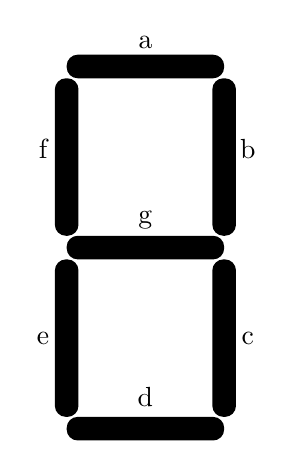
\begin{tikzpicture}[line join=round, line cap=round, rounded corners, ultra thick]
        % segments
        \fill[black] (0.15,0) rectangle +(2,0.3);   % a
        \fill[black] (0,0) rectangle +(0.3,-2); % f
        \fill[black] (2,0) rectangle +(0.3,-2); % b
        \fill[black] (0.15,-2.) rectangle +(2,-0.3);   % g
        \fill[black] (0,-2.3) rectangle +(0.3,-2);  % e
        \fill[black] (2,-2.3) rectangle +(0.3,-2);  % c
        \fill[black] (0.15,-4.3) rectangle +(2,-0.3);   % g
        % labels
        \node[align=center] at (1.15,0.45) {a};
        \node[align=center] at (1.15,-1.8) {g};
        \node[align=center] at (1.15,-4.05) {d};
        \node[align=center] at (-0.15,-0.9) {f};
        \node[align=center] at (-0.15,-3.3) {e};
        \node[align=center] at (2.45,-0.9) {b};
        \node[align=center] at (2.45,-3.3) {c};
    \end{tikzpicture}
\caption{Seven segment LED display segments are labeled as shown.}
\label{fig:ledsegments}
\end{figure}


\begin{figure}[!htb]
	\centering
	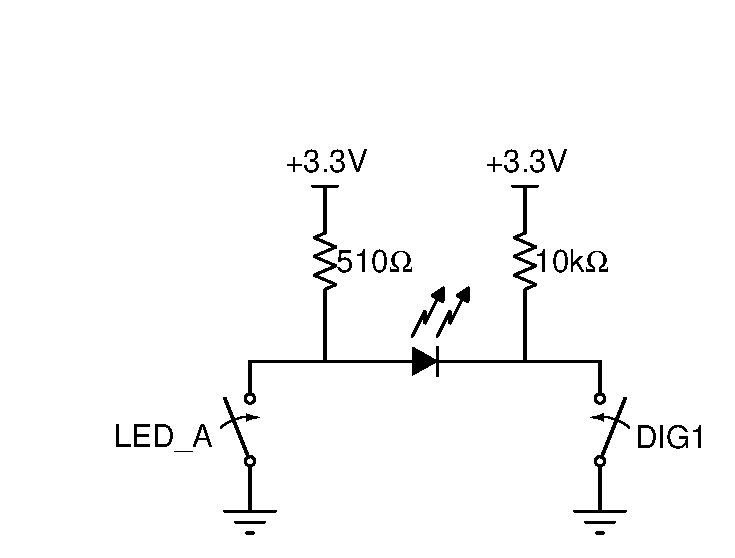
\includegraphics{i2cgpio/7SegCircuit.eps}
    \caption{A single segment of a seven segment digit is connected with this circuit. 
        Setting LED\_A to 1 (open) and DIG1 to 0 (closed) lights up the segment.}
    \label{fig:sevensegindcircuit}
\end{figure}

\begin{figure}[!htb]
	\centering
	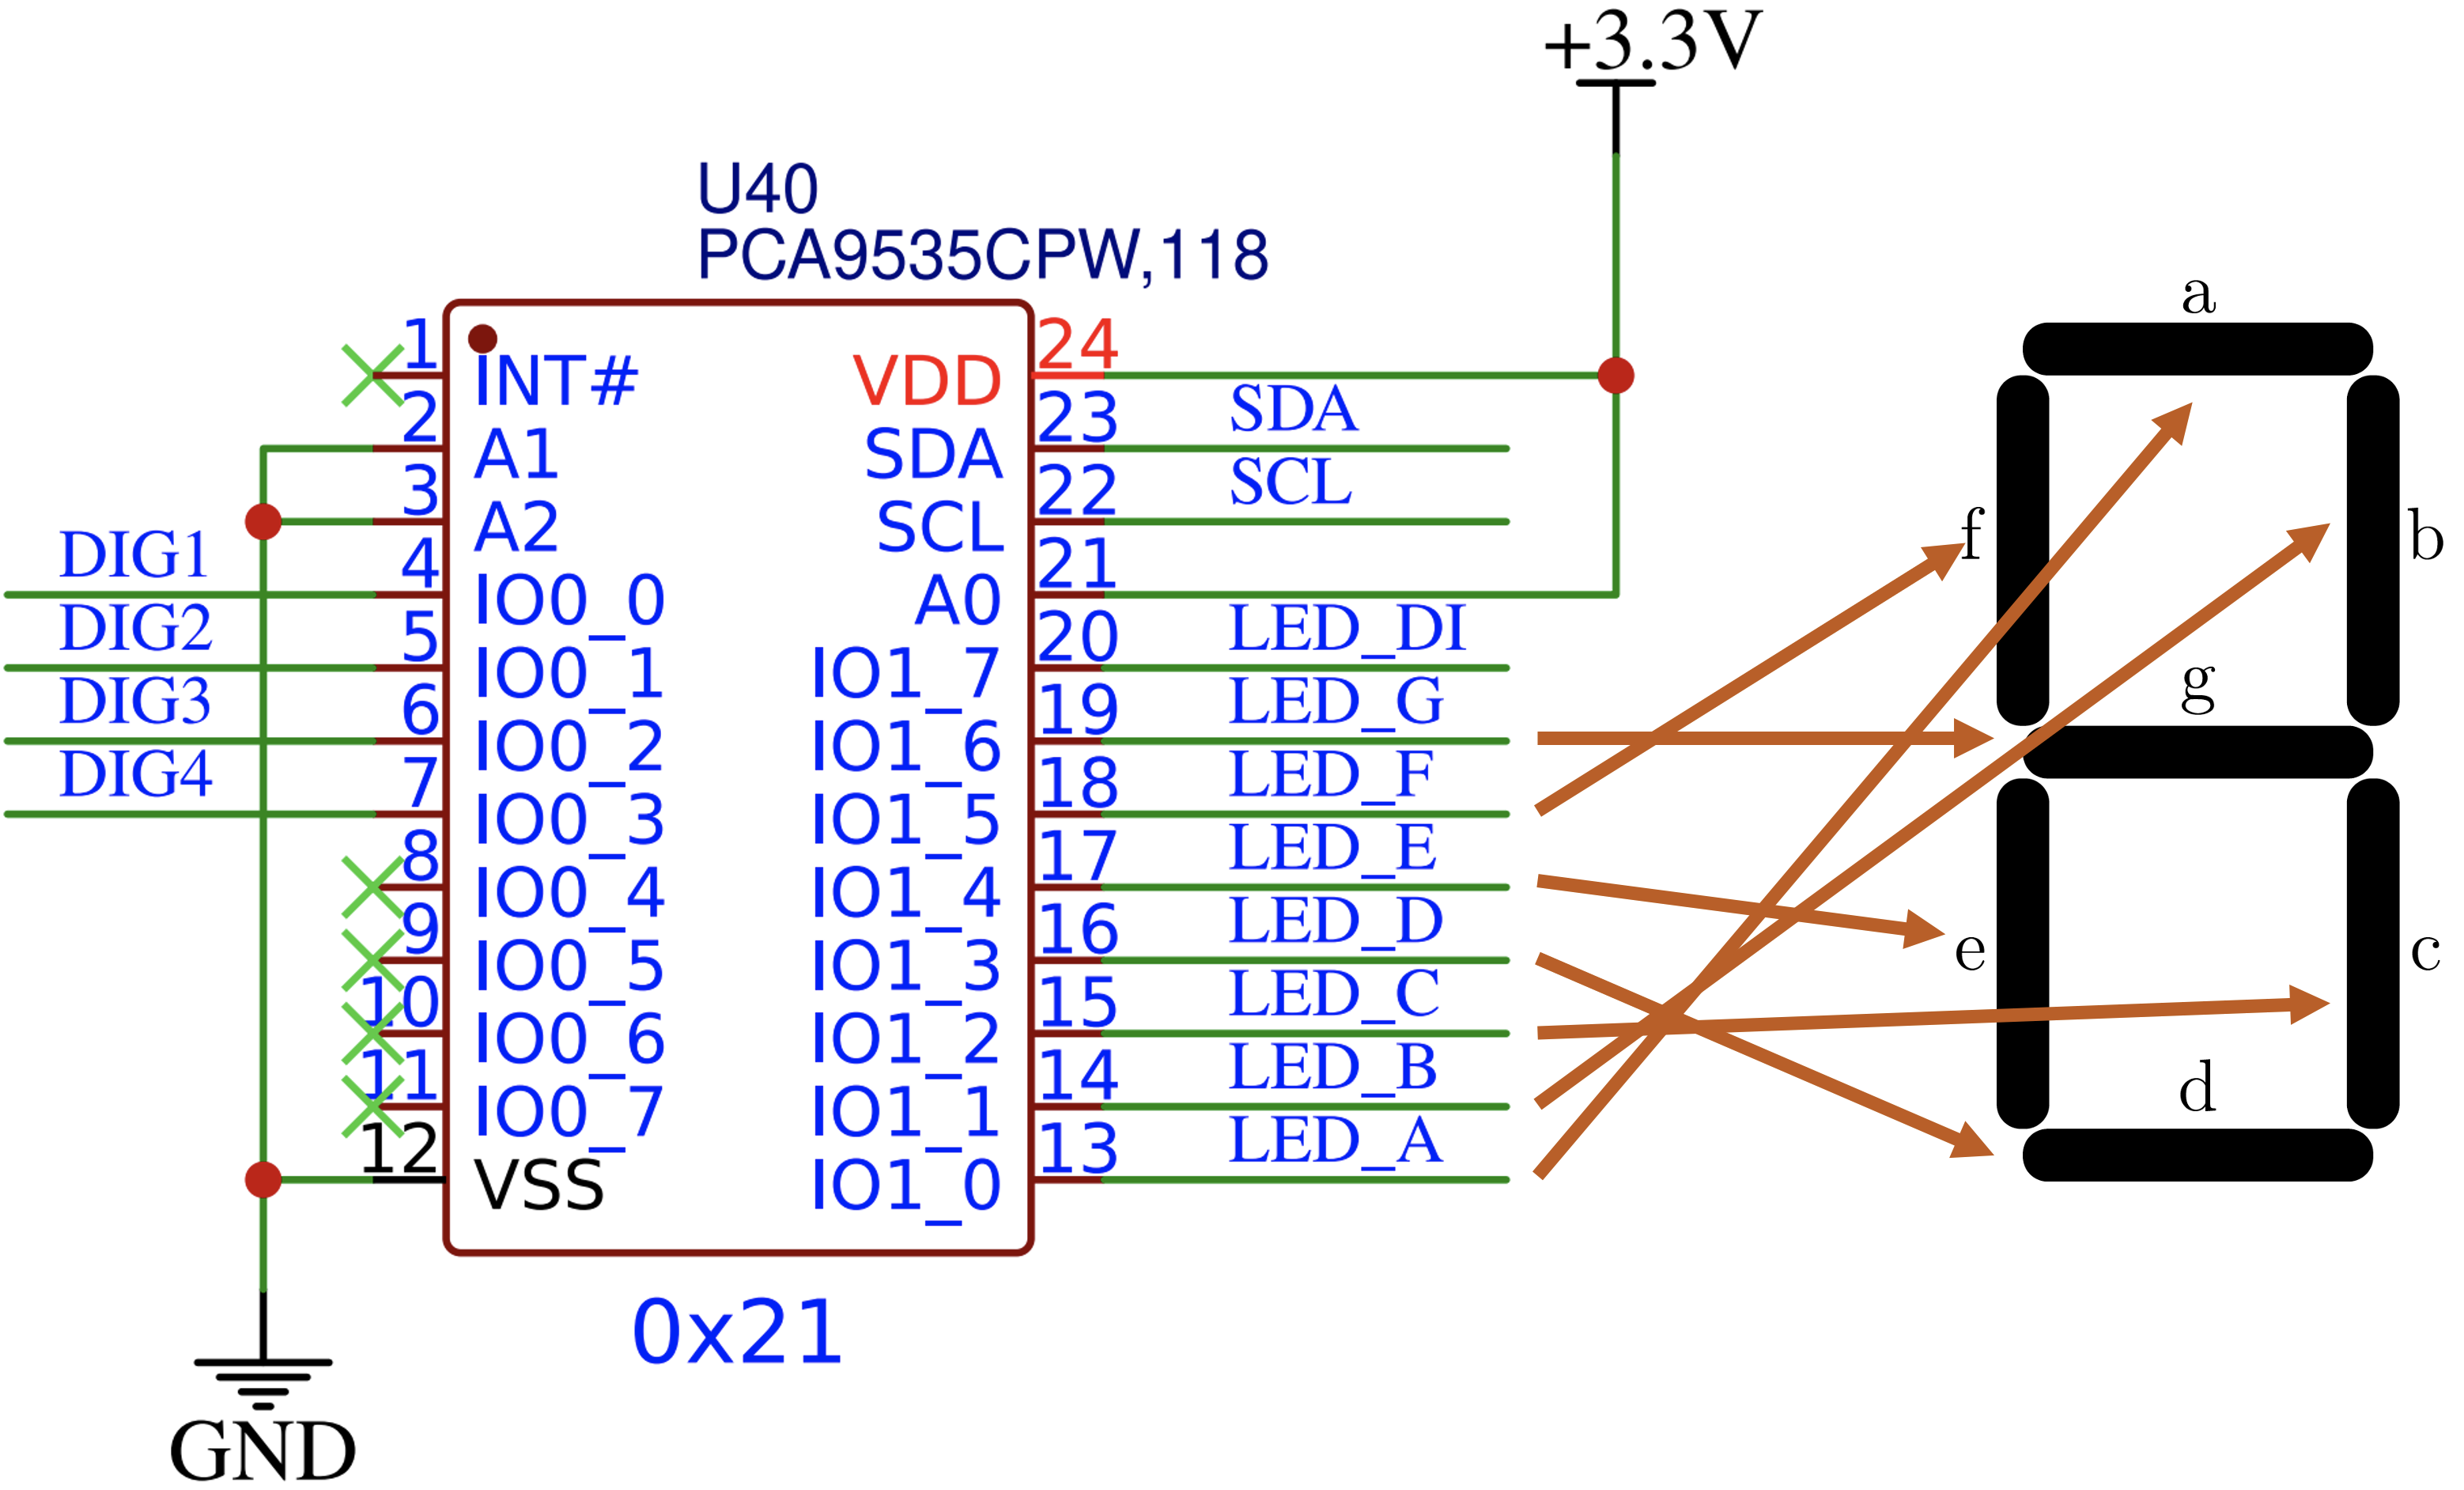
\includegraphics[scale=0.23]{i2cgpio/PCA9535-Segs.png}
    \caption{This shows the mapping between the PCA9535 at address 0x21 and 
    the seven segment display segments.}
    \label{fig:PCA9535Segs}
\end{figure}

\begin{figure}[!htb]
	\centering
	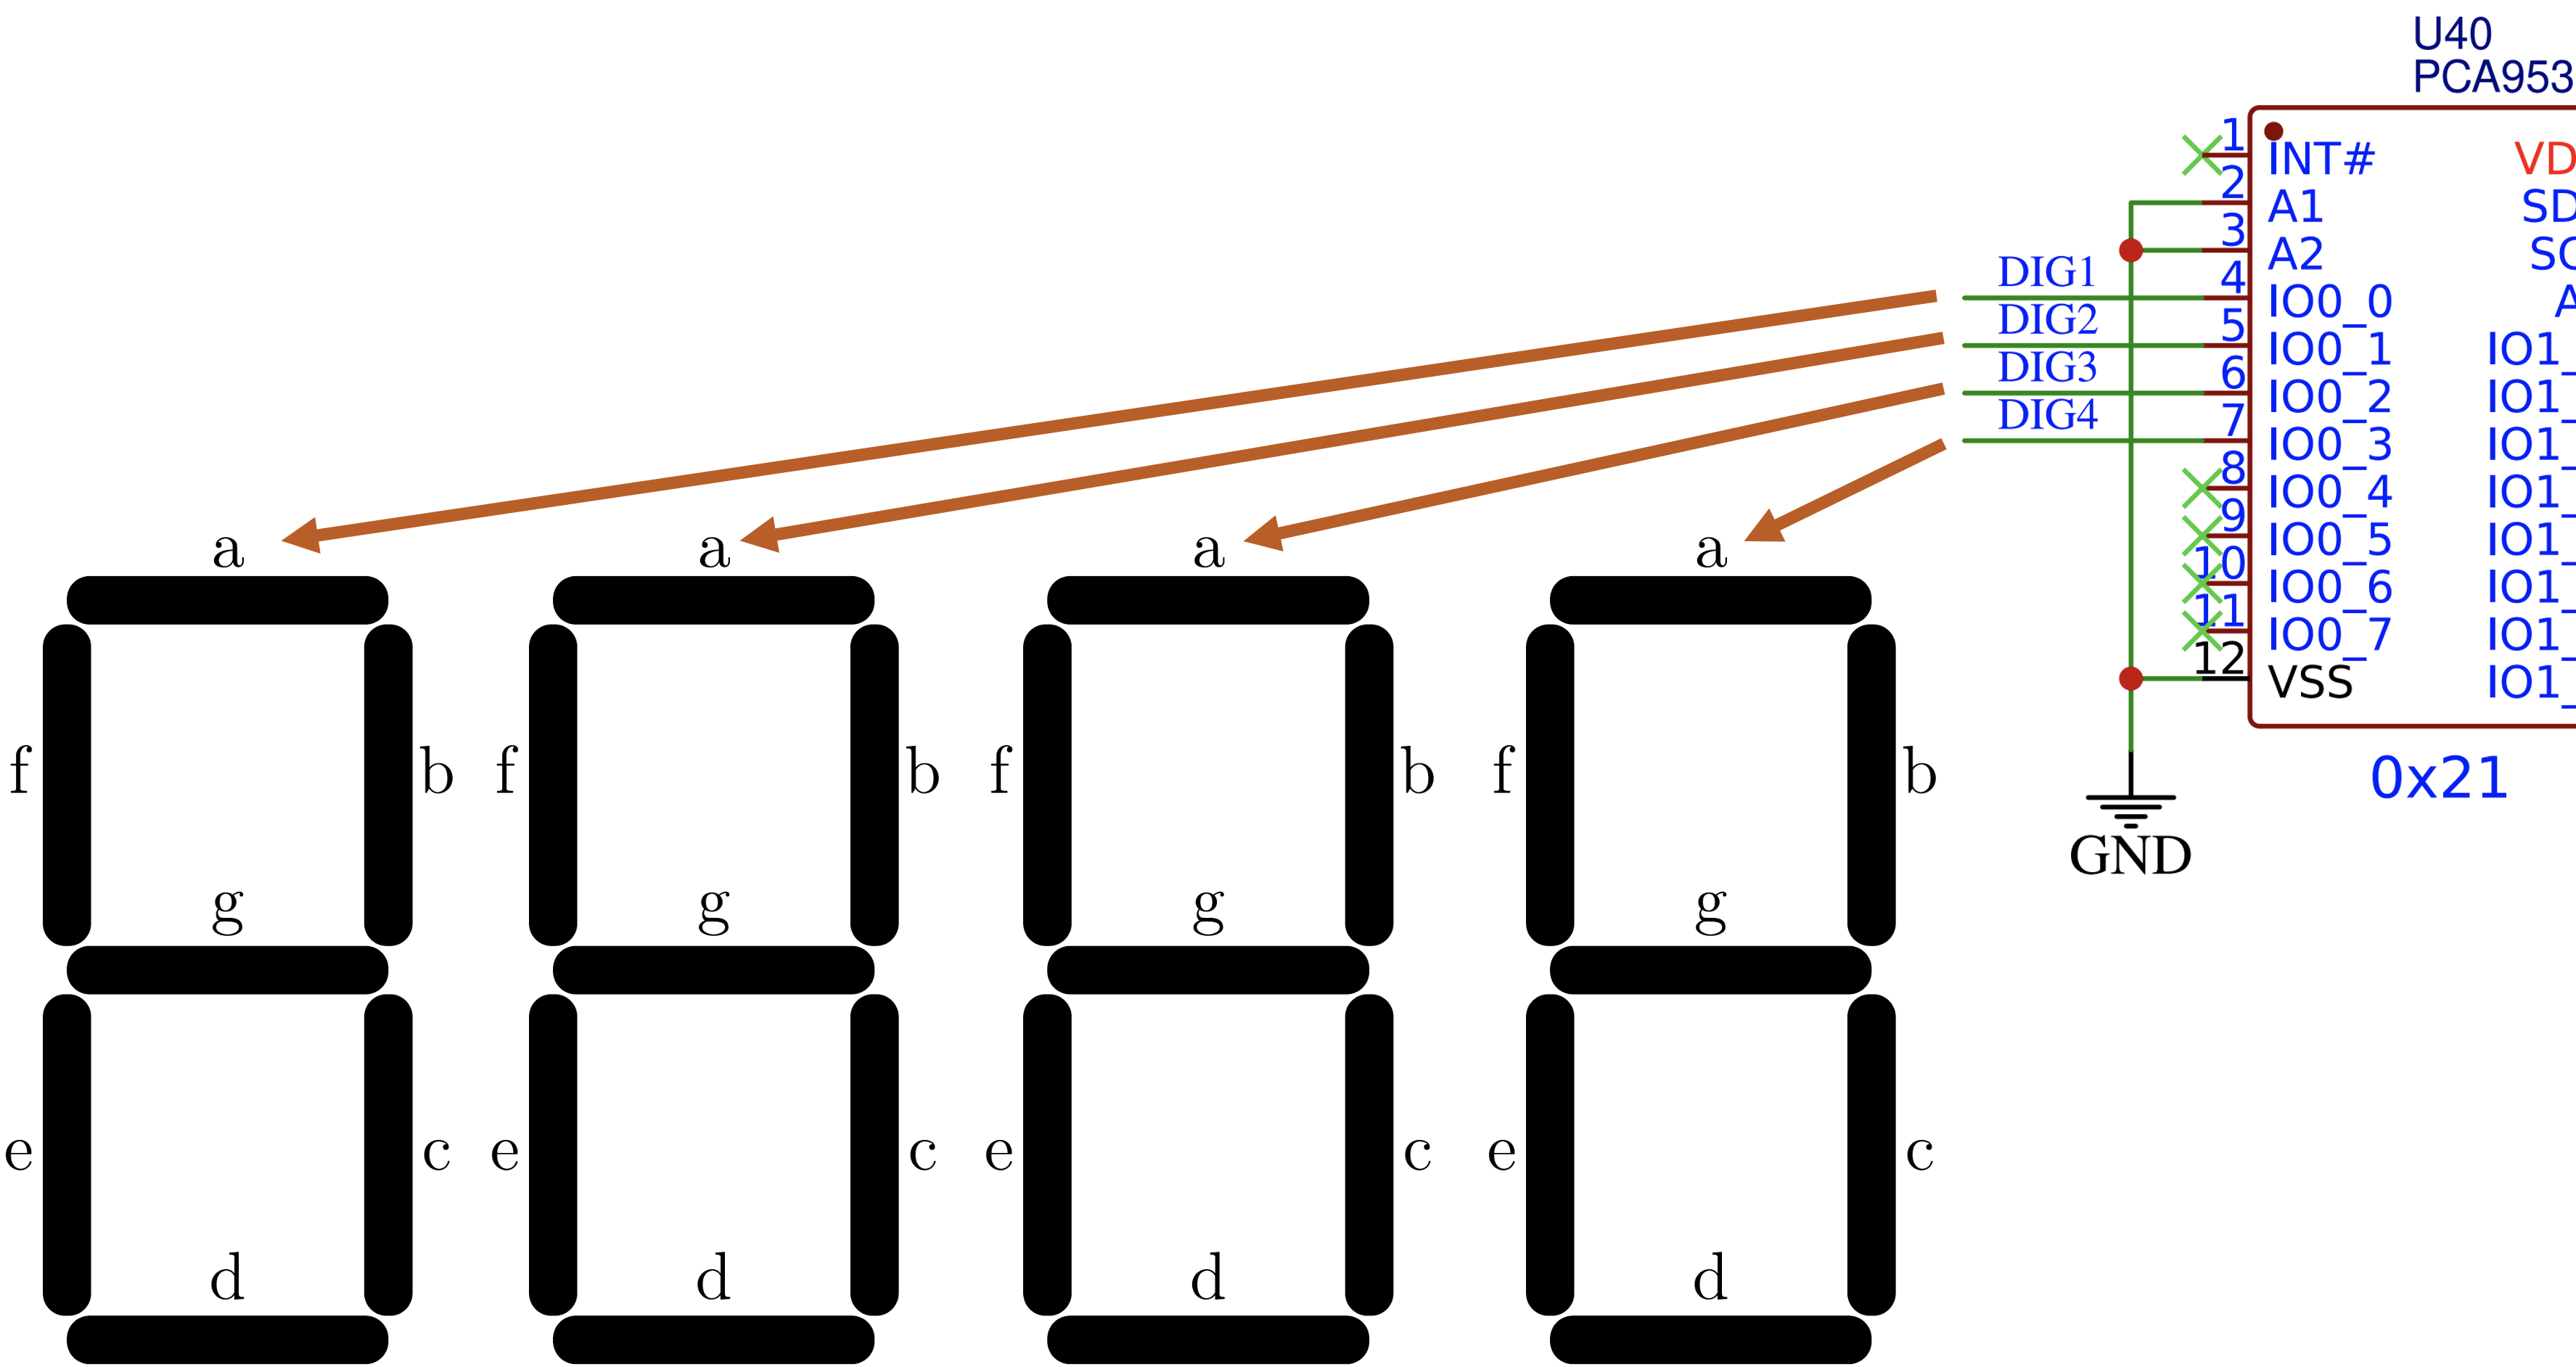
\includegraphics[scale=0.2]{i2cgpio/PCA9535-Digs.png}
    \caption{This shows the mapping between the PCA9535 at address 0x21 and 
    the seven segment display digits.}
    \label{fig:PCA9535Digs}
\end{figure}

\begin{figure}[!htb]
	\centering
	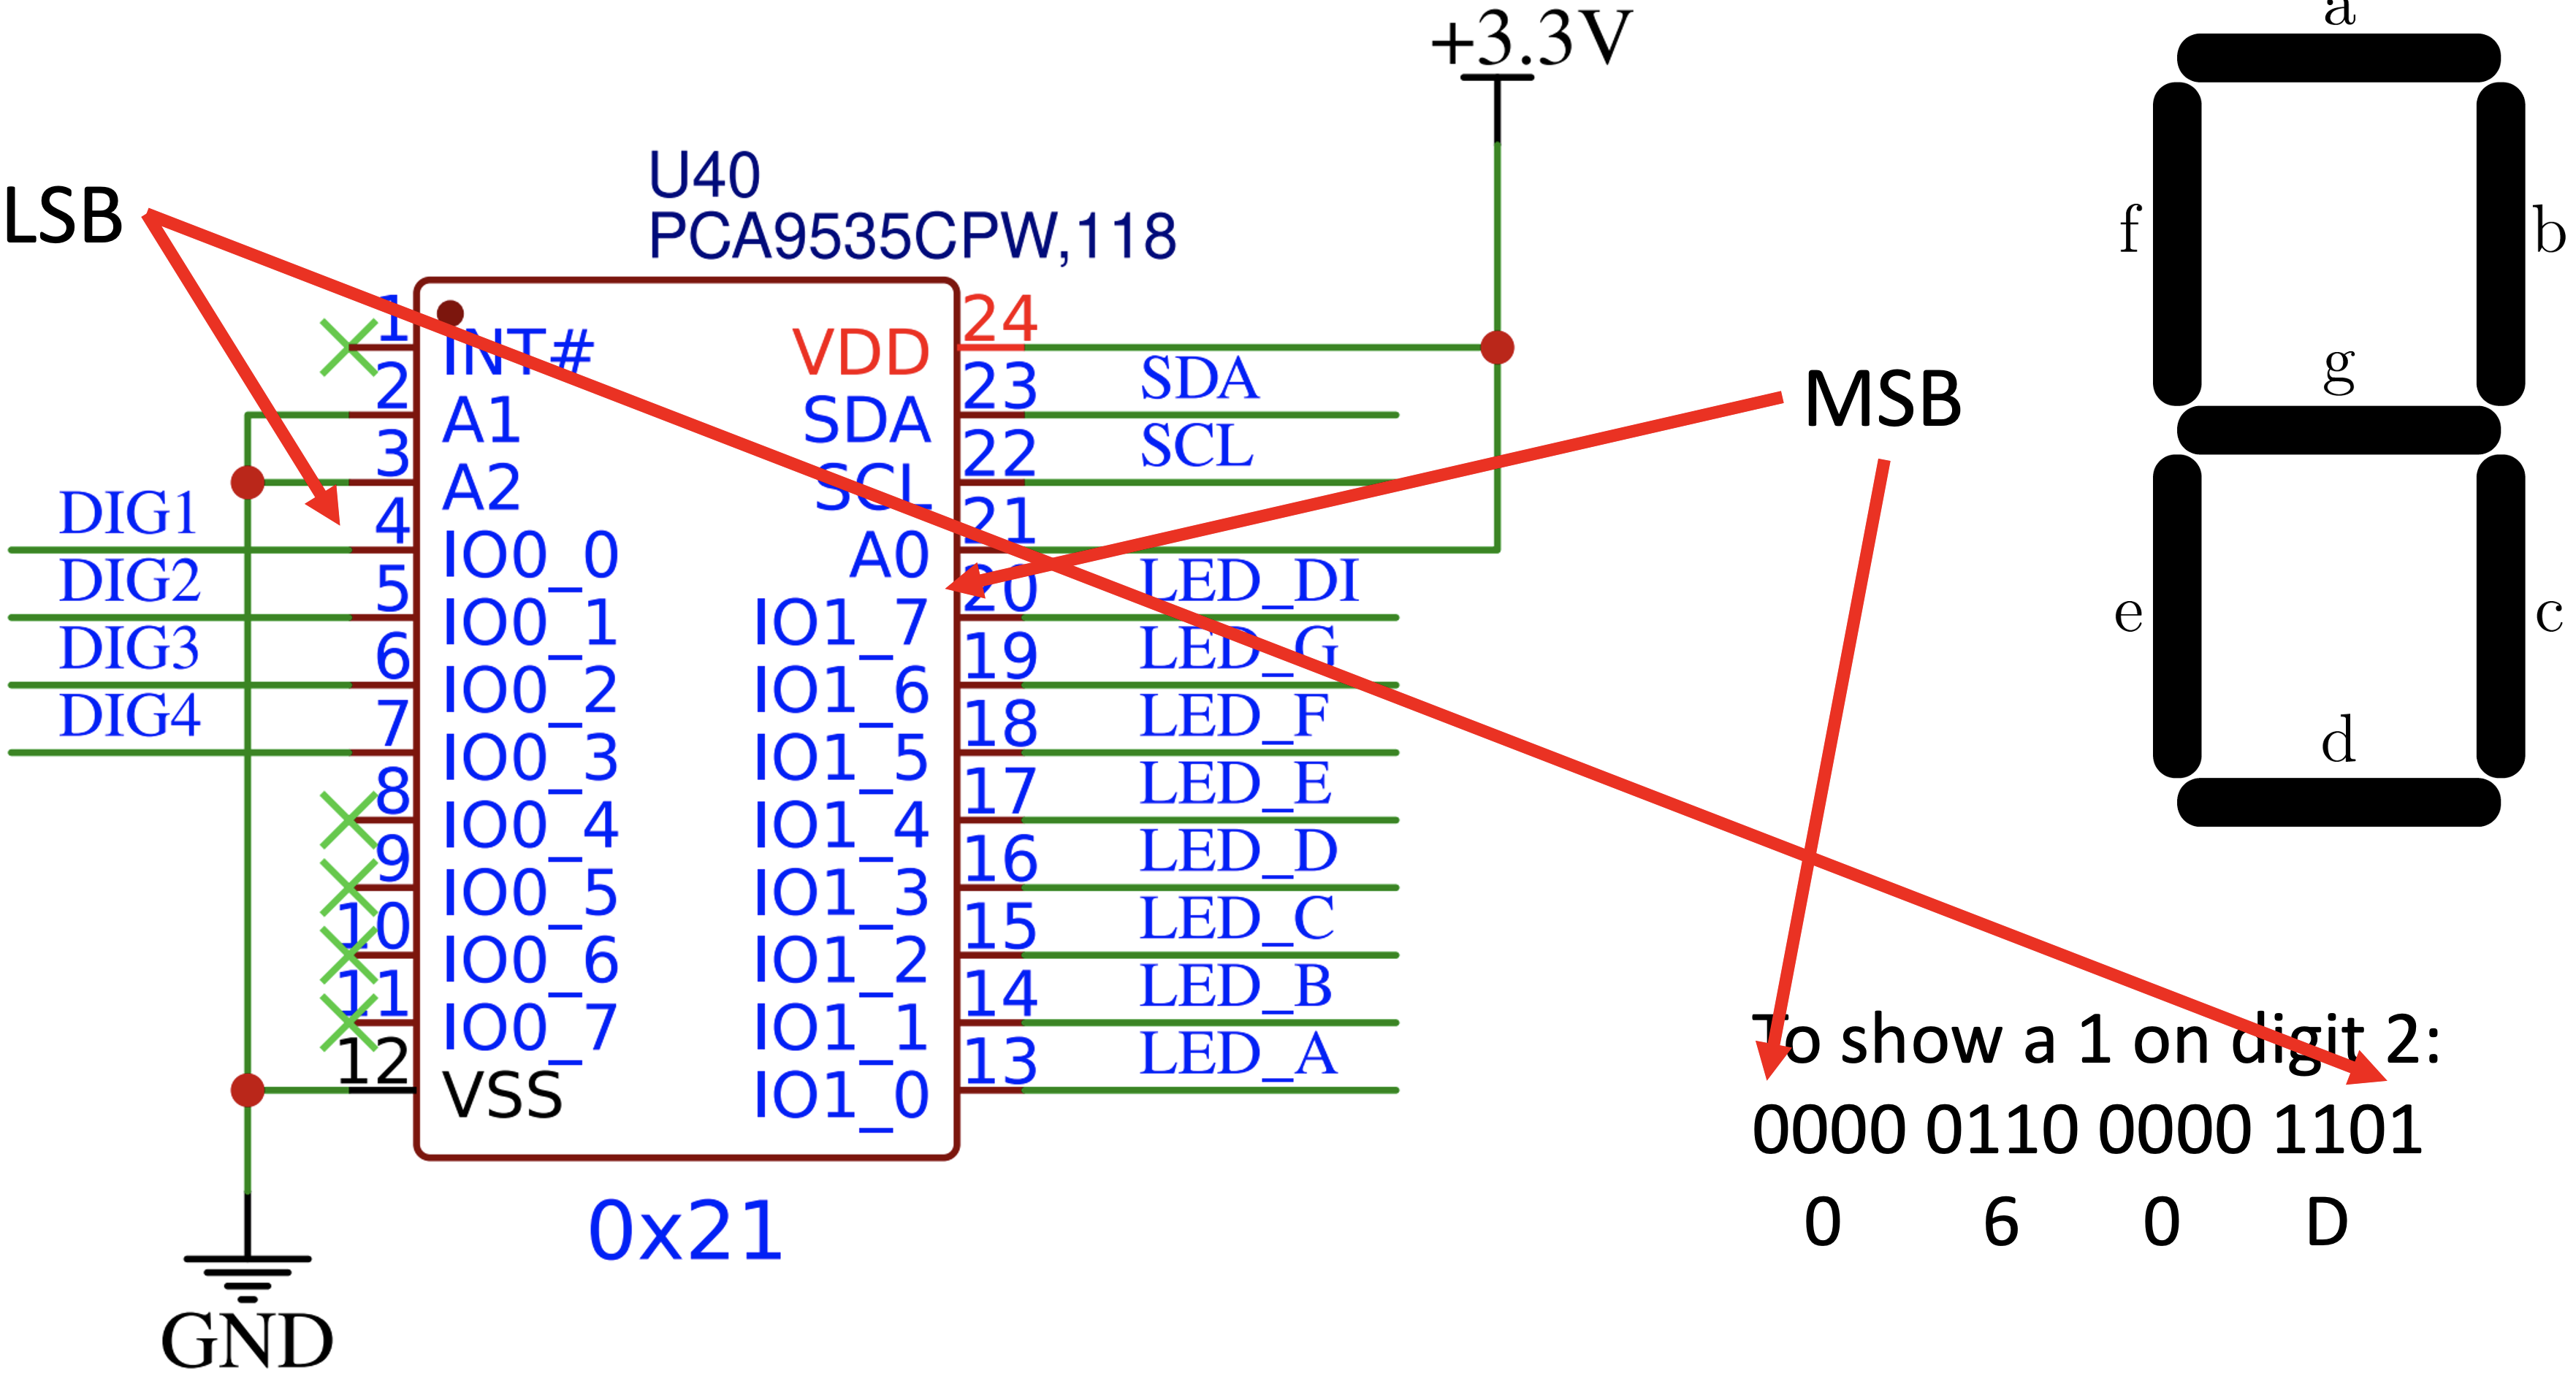
\includegraphics[scale=0.2]{i2cgpio/PCA9535-LSB-MSB.png}
    \caption{This shows the mapping between the PCA9535 at address 0x21 and 
    the seven segment display showing most significant and least significant digits.}
    \label{fig:PCA9535LSB}
\end{figure}
